\label{sec:CKM_prospects}

Weak charged currents mix quarks of different generations. In the SM, the strengths of the corresponding transitions are encoded in the unitary Cabibbo-Kobayashi-Maskawa (CKM) matrix~\cite{Cabibbo:1963yz,Kobayashi:1973fv}.
Unitarity, in conjunction with invariance under field redefinitions, implies that all nine complex elements of the  $3\times 3$ CKM matrix are described by four physical parameters. 
In turn, this implies relations between different CKM elements, such as the closure of the standard CKM unitarity triangle (which may not hold  in the presence of new physics).  
Overconstraining the apex of the unitarity triangle from tree- and loop-level quark mixing processes is therefore a powerful way to probe for virtual new physics effects that may arise from mass scales above those which can be directly searched for at colliders. In many cases such indirect probes of new physics will not be limited by either experimental or theoretical systematics at least in the {\bf mid-term}, i.e., in the \HLLHC era, and potentially even for any {\bf long-term} programs (see Table \ref{table:Proj} for expected improvements in lattice QCD for a selection of observables).


\begin{table}
\caption{Current estimates and projections for experimental reach for a selection of observables at Belle~II and LHCb, including Upgrade~II, compared to lattice QCD determinations of hadronic inputs for the {\bf short-} and {\bf mid-term}, taken to be, respectively, the Phase I and II stages defined in Ref.~\cite{Cerri:2018ypt}. It is assumed that the QED corrections to lattice QCD results will be calculated. For a more complete listing of lattice QCD projections see Table 42 of Ref.~\cite{Cerri:2018ypt}.}
    \label{table:Proj}
    {\footnotesize
\begin{center}
\begin{tabular}{ccccc}
\hline\hline
Quantity & Ref. &present error & short-term & mid-term\\
\hline
$(\Delta m_s/\Delta m_d)_{\rm exp}$ & \cite{Tanabashi:2018oca} & $0.4\%$ & - & -
\\
$\xi$ for $(\Delta m_s/\Delta m_d)_{\rm theor}$ & \cite{Cerri:2018ypt} & $1.4\%$ & $0.3\%$ & $0.3\%$
\\
\hline
$B\to \pi$: $|V_{ub}|_{{\rm exp}}$ & \cite{Cerri:2018ypt,Bediaga:2018lhg,Kou:2018nap} &    $2.3\%$ & $1.6\%$ & $1.1\%$\\
$B\to \pi$: $|V_{ub}|_{{\rm theor}}$ & \cite{Cerri:2018ypt} &    $2.9\%$ & $1\%$ & $1\%$\\
\hline
$B\to D$: $|V_{cb}|_{{\rm exp}}$& \cite{Cerri:2018ypt,Kou:2018nap} &   $ 2.0\%$ & $1.4\%$ & -\\
$B\to D$: $|V_{cb}|_{{\rm theor}}$&\cite{Cerri:2018ypt} &    $1.4\%$ & $0.3\%$ & $0.3\%$\\
\hline
$B\to D^*$: $|V_{cb}|_{{\rm exp}}$ & \cite{Kou:2018nap}& $1.2\%$ &- & - \\ 
$B\to D^*$: $|V_{cb}|_{{\rm theor}}$ & \cite{Cerri:2018ypt}& $1.4\%$ & $0.4\%$ & $0.4\%$ \\  
\hline
$\Lambda_b\to p(\Lambda_c)$: $|V_{ub}/V_{cb}|_{{\rm exp}}$ & \cite{Bediaga:2018lhg} &   $ 6\%$ & $1\%$ & $1\%$\\
$\Lambda_b\to p(\Lambda_c)$: $|V_{ub}/V_{cb}|_{{\rm theor}}$  &\cite{Cerri:2018ypt} & $4.9\%$ & $1.2\%$ & $1.2\%$\\
\hline
\hline
\end{tabular}
\end{center}
}
\end{table}

\begin{table}
\caption{Relative uncertainties on the predictions of UT parameters and angles, using current and extrapolated input values for measurements and theoretical parameters (UTfit collaboration, from~\cite{Cerri:2018ypt}, with short-(mid-)term taken as Phase I(II) stages defined in~\cite{Cerri:2018ypt}).}
\label{tab:utfit_global}
{\footnotesize
 \begin{center}
       \begin{tabular}{ccccccccc}
               \hline\hline
                & $\lambda$ & $\bar{\rho}$ & $\bar{\eta}$ & $A$ & $\sin2\beta$ & $\gamma$ & $\alpha$ & $\beta_s$ \\ \hline
                       Current &0.12\%& 9\% & 3\% & 1.5\% & 4.5\% & 3\% & 2.5\% & 3\% \\
                       short-term  &0.12\%& 2\% & 0.8\% & 0.6\% & 0.9\% &  0.9\% & 0.7\% & 0.8\%\\
                       mid-term  &0.12\%& 1\% & 0.6\% & 0.5\% & 0.6\% & 0.8\% & 0.4\% & 0.5\%\\ \hline
       \hline
       \end{tabular}
\end{center}
}
\end{table}



Figure~\ref{fig:UTprojection} shows the projected {\bf short-} and {\bf mid-term} improvements on constraints in the plane of two unitarity triangle parameters, $\bar{\rho}$ and $\bar{\eta}$, using only expected improvements in LHCb inputs and lattice-QCD calculations, while Table \ref{tab:utfit_global} gives the expected improvements by using both LHCb and Belle-II results. The increased sensitivity will allow for extremely precise tests of the CKM paradigm. In particular, it will permit the tree-level observables, which provide the SM benchmarks, to  be assessed against  those with loop contributions, which are more susceptible to new physics.  In practice, this already very powerful ensemble of constraints will be 
further strengthened by complementary measurements from Belle II, particularly in the case of $|V_{ub}|$ and $|V_{cb}|$, where $\sim $1\% precision is expected. Improvement on the determination of $|V_{cb}|$ will also greatly impact the constraints on the CKM matrix elements that follow from the measurement of $\varepsilon_K$.

\begin{figure}[t]
\begin{center}
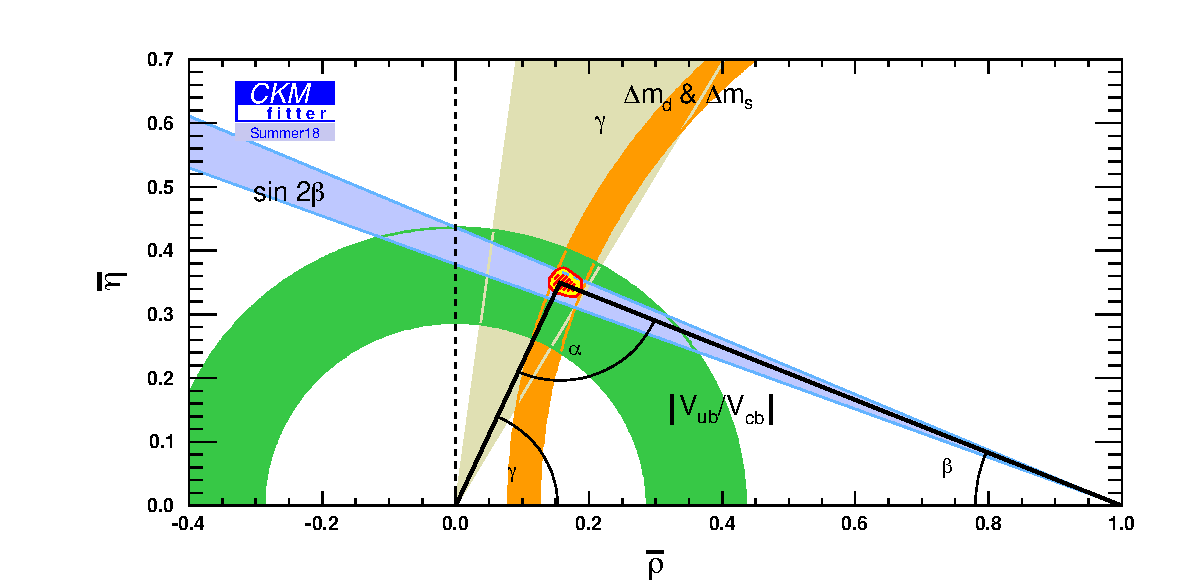
\includegraphics[width=0.65\textwidth]{Flavour/figs/rhoeta_small_LHCb_Summer18.pdf}

\begin{minipage}{0.65\textwidth}
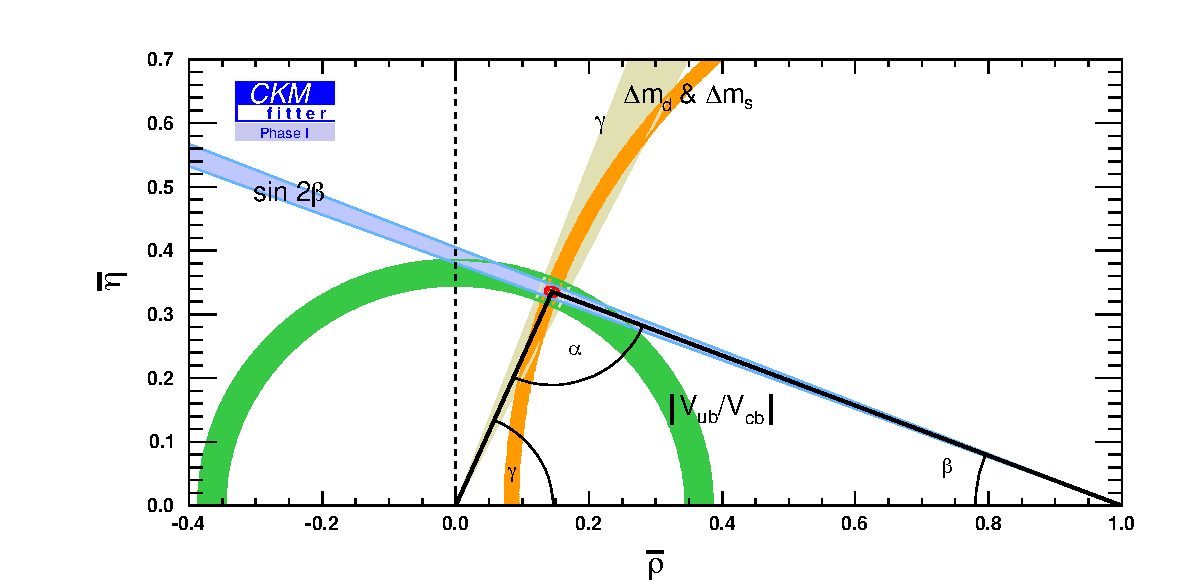
\includegraphics[width=\textwidth]{Flavour/figs/rhoeta_small_LHCb_Stage1.pdf}\vspace{-5.36cm}
\mbox{\hspace{7.9cm}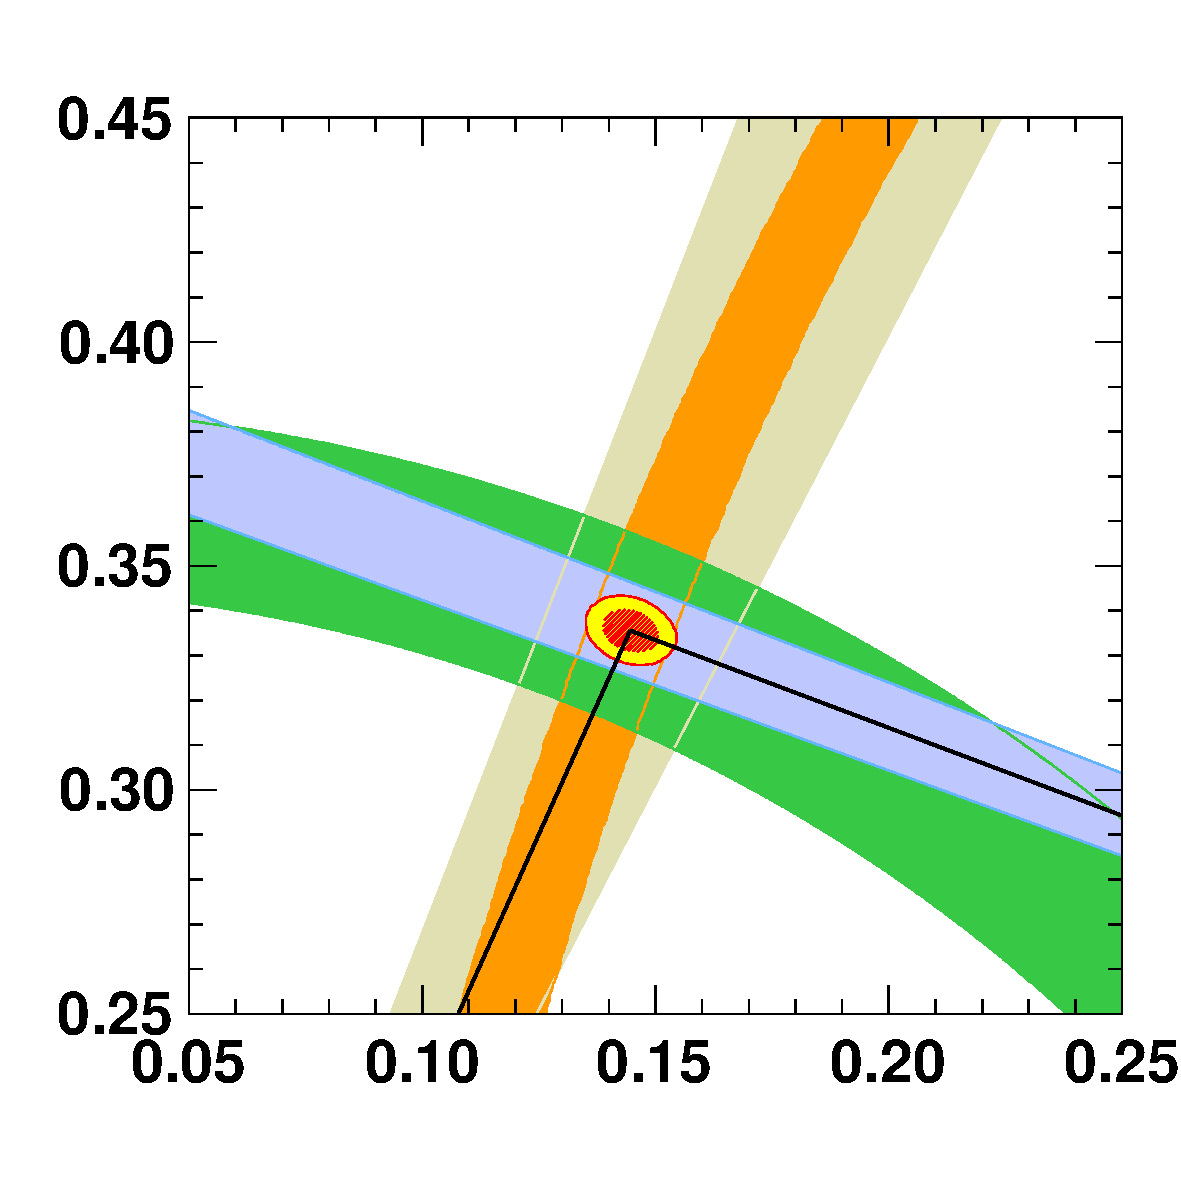
\includegraphics[width=0.26\textwidth]{Flavour/figs/rhoeta_small_zoom_LHCb_Stage1.pdf}}
\vspace{2.25cm}
\end{minipage}

\begin{minipage}{0.65\textwidth}
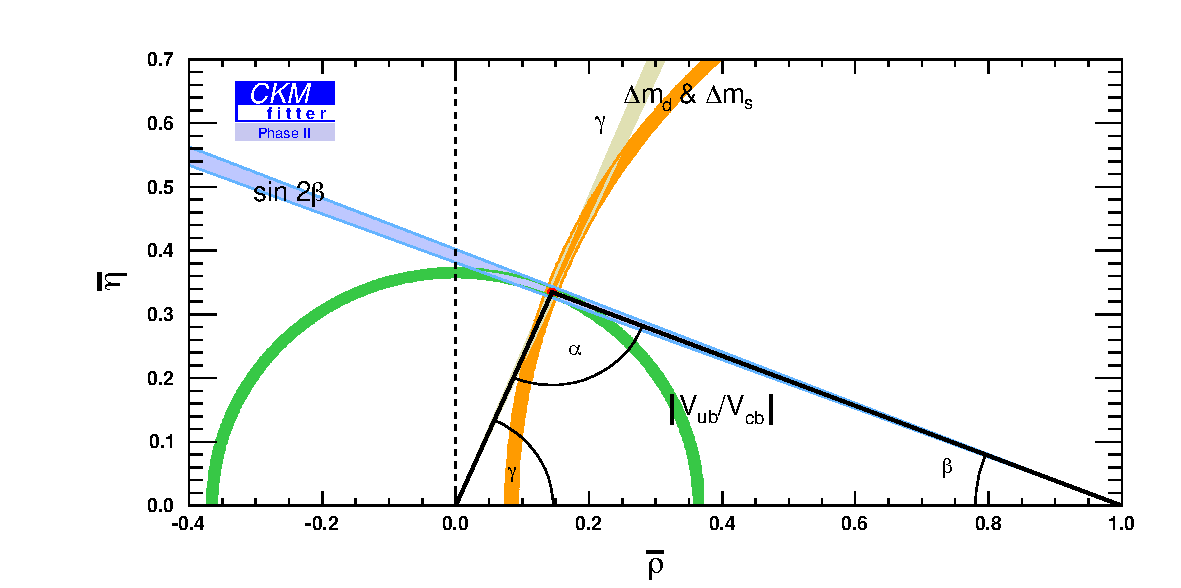
\includegraphics[width=\textwidth]{Flavour/figs/rhoeta_small_LHCb_Stage2.pdf}\vspace{-5.36cm}
\mbox{\hspace{7.9cm}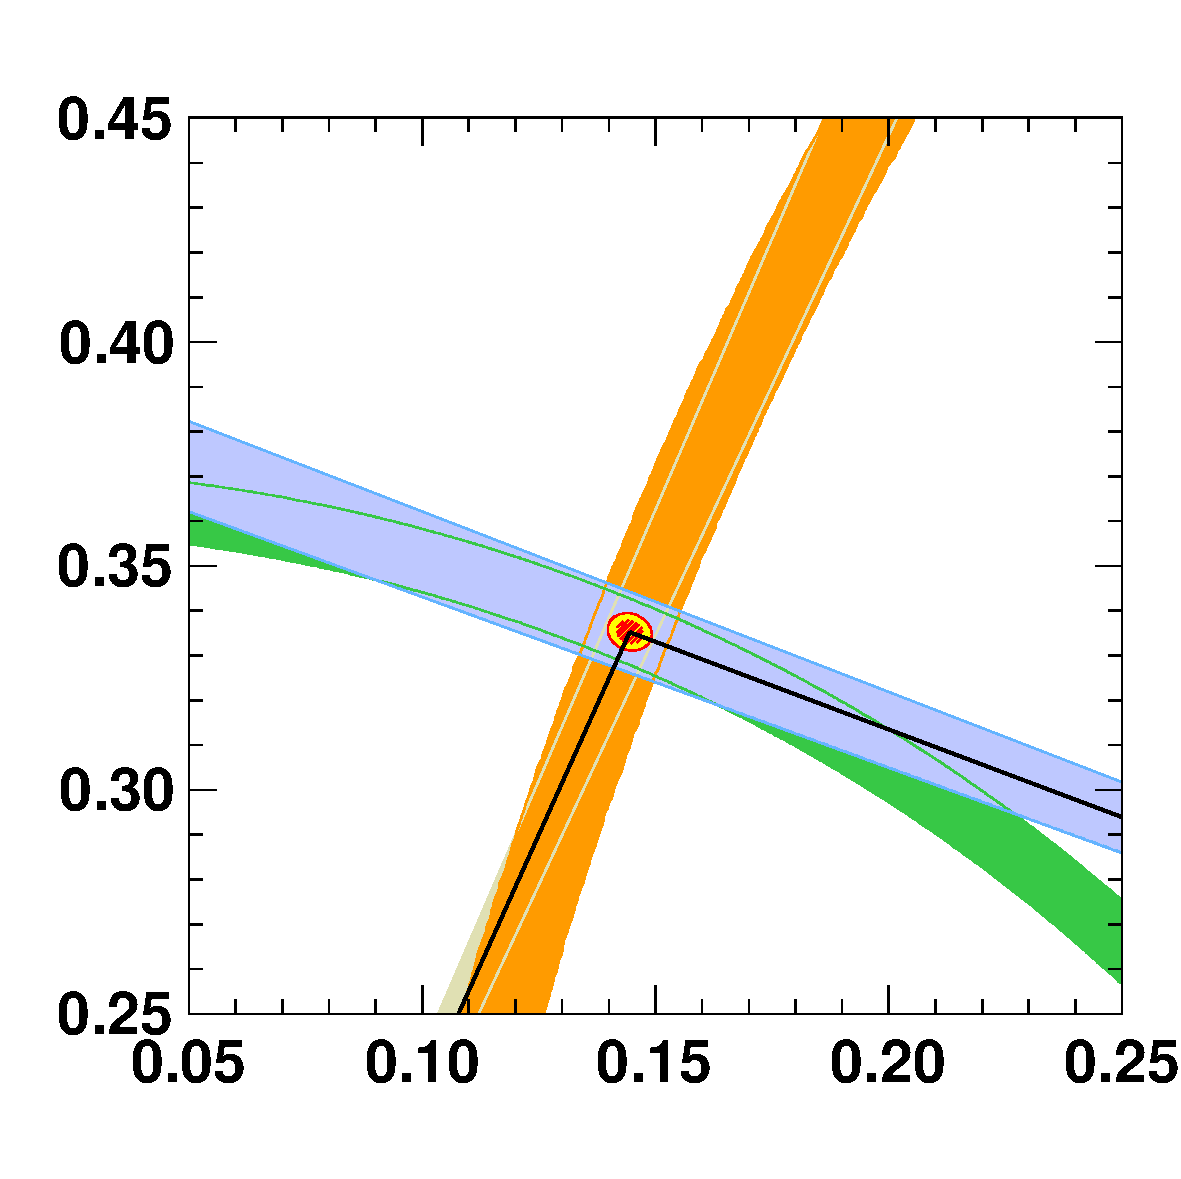
\includegraphics[width=0.26\textwidth]{Flavour/figs/rhoeta_small_zoom_LHCb_Stage2.pdf}}
\vspace{2.25cm}
\end{minipage}

\caption{\small  Evolving constraints in the $\bar{\rho}-\bar{\eta}$ plane from LHCb measurements and lattice QCD calculations, alone, with current inputs (2018), and the anticipated improvements from the data accumulated by 2025  (23\,fb$^{-1}$) and 2035 (300\,fb$^{-1}$), from top to bottom, respectively.
Figures from Ref.~\cite{Bediaga:2018lhg}. }
\label{fig:UTprojection}
\end{center}
\end{figure} 

The \textbf{angle} $\pmb{\gamma}$ is currently the least well known CKM parameter ($\pm 5^\circ$).
In the {\bf short-term} both LHCb Upgrade~I and Belle ~II will provide measurements at $\sim$ 1.5 $^\circ$. In the {\bf mid-term} LHCb Upgrade~II will allow for a  sensitivity at the sub-degree level.
The best sensitivity to $\gamma$ is from $B\to DK$ decays. The anticipated largest systematic uncertainty will be due to the external inputs on the strong phase differences in $D$ meson decays, for which 
BES~III and the SCT factories are expected to provide precise measurements.  Table~\ref{tab:utfit_global} shows the foreseen {\bf mid-term} impact of experimental and theoretical developments on global CKM fits, as estimated by the UTFit group~\cite{Cerri:2018ypt} (comparable CKMfitter estimates can also be found in Ref.~\cite{Cerri:2018ypt}).

The precision measurement of the $B_s$ weak mixing phase, $\phi_s$, will be another highlight of the {\bf mid-term} programme. The expected precision on $\phi_s^{c\bar{c}s}$ at the end of \HLLHC  will be $\sim 5$~mrad for ATLAS and CMS, and $\sim 3$~mrad for LHCb. 
This determination of $\phi_s$ from a loop induced process susceptible to new physics, will be at the same level of precision as the current one on the indirect determination (based on the CKM fit using tree-level measurements). This allows for a precise probe of new physics contributions.





